\section*{Platinsponsor und Aussteller}

\vspace{-0.5cm}
\centerline{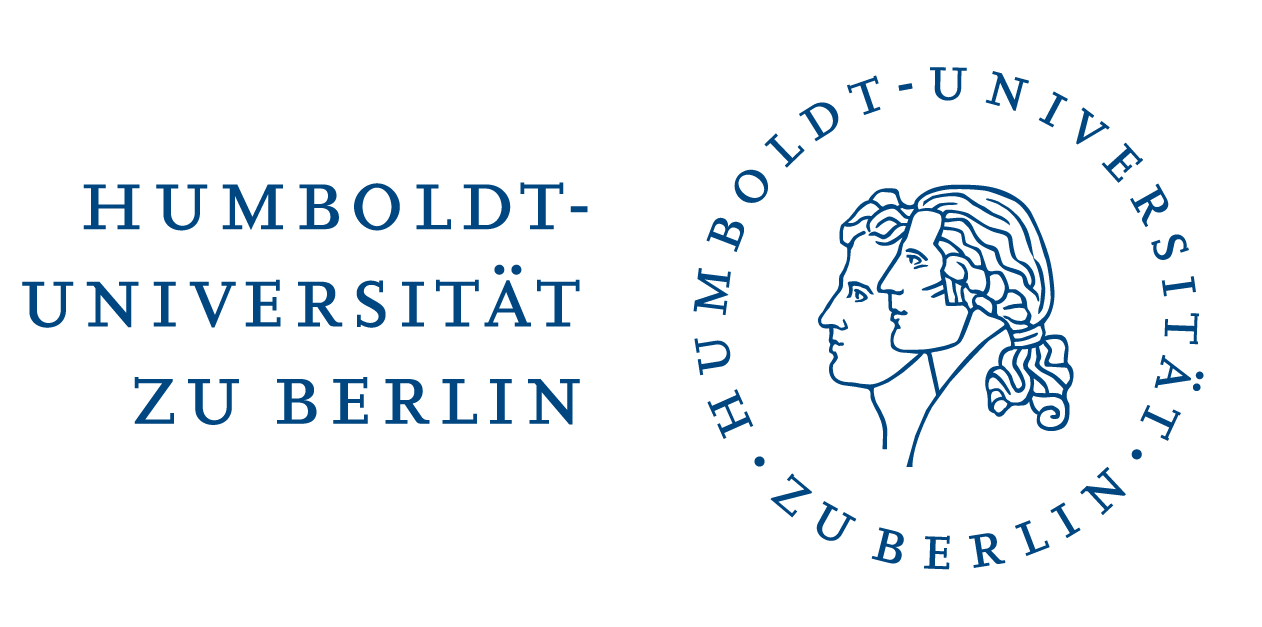
\includegraphics[width=0.5\textwidth]{003_hu_siegel-kombi_rgb.png}}
Die Humboldt-Universität zu Berlin, gegründet 1810, ist die älteste Hochschule in Berlin
und eine der renommiertesten Universitäten weltweit. Das Lehr- und Forschungsangebot der HU umfasst heute alle grundlegenden
Wissenschaftsdisziplinen der Geistes-, Sozial- und Kulturwissenschaften, der Rechtswissenschaften, der Lebenswissenschaften, der Mathematik und Naturwissenschaften, der Medizin, der Agrarwissenschaften und der Nachhaltigkeits- und Antikeforschung. Aktuell studieren an der Humboldt-Universität fast 37\,000 junge Menschen aus über 100 Ländern in 171 Bachelor- und Masterstudiengängen betreut von über 400 Professor:innen. Zirka 34 Prozent der wissenschaftlichen Mitarbeiter:innen kommen aus anderen Ländern. Aufgrund zahlreicher Projekte der Spitzenforschung und renommierter internationaler Netzwerke ist die Humboldt-Universität eine der bedeutendsten Universitäten im deutschsprachigen Raum. Bei der Exzellenzstrategie 2019 wurde sie gemeinsam mit den Partner:innen der Berlin University Alliance als Exzellenzverbund ausgezeichnet. Zuvor gehörte sie seit 2012 zu einer der elf deutschen Exzellenzuniversitäten. Die HU verbindet Forschungsexzellenz mit innovativer Nachwuchsförderung. Im Fokus der Lehre stehen forschendes Lernen, Interdisziplinarität und Internationalisierung.
